\documentclass[12pt,twoside,a4paper]{article}
\usepackage[utf8]{inputenc}
\usepackage[T1]{fontenc}
\usepackage[german]{babel}
\usepackage{amsmath}
\usepackage{paralist}
\usepackage{graphicx}
\usepackage{float}
\usepackage{caption}
\usepackage{multirow,tabularx}
\usepackage{units}

\title{Auswertung Wärmestrahlung}
\author{Jonas Müller}
\date{28.06.14}

\begin{document}

\section{Stefan-Boltzmann-Gesetz}

In diesem Versuch sollte die Gültigkeit des Stefan-Boltzmann-Gesetzes überprüft werden. Dieses lautet wie folgt:

\begin{equation*}
P = \sigma \cdot A \cdot T^4
\end{equation*}

Konkret wollen wir die $T^4$-Abhängigkeit der abgestrahlten Leistung nachweisen.\\
Dazu wurde ein schwarzer Strahler so auf einer Schiene befestigt, dass die Öffnung des Strahlers entlang der Schiene ausgerichtet war. Der Strahlung wurde mit eine Stromquelle verbunden und so erhitzt. Über ein Thermoelement wurde die Temperatur des Strahlers registriert, wobei allerdings nicht die Temperatur direkt, sonder eine Spannung gemessen wurde. Mit einer gegebenen Umrechnungstabelle lässt sich aus der Spannung die entsprechende Temperatur bestimmen. Wie in der Vorbereitung erwähnt diente eine Mollsche Thermosäule dazu die Strahlung zu messen. Damit sich diese nicht zu stark erhitzt und der Messfehler somit größer wird, wurde davor noch eine Lochblende auf der Schiene montiert. Wir nahmen in nach unterschiedlich großen Zeitintervallen jeweils die Temperatur (bzw. die Spannung $U_{Th}$) und die Spannung $U_P$, welche an der Thermosäule gemessen wurde, auf. Dabei wurde die Thermosäule zwischen den Messungen mit einer reflektierenden Platte abgeschirmt. Dadurch soll verhindern werden, dass zwischen den Messungen Strahlung auf die Thermosäule trifft und so mit die Anfangstemperatur verändert. In der Vorbereitung wurde bereits erläutert, dass gilt:

\begin{equation*}
U_P \sim T^4
\end{equation*}

Weshalb können wir direkt die gemessenen $U_P$-Werte nutzen um die $T^4$-Abhängigkeit zu zeigen. Während des Versuchs steigerten wir die Spannung zum erhitzen des Strahlers in mehreren Schritten von ca. $\unit[30]{V}$ auf ca. $\unit[65]{V}$, damit wir nicht zu lange zwischen den Messungen warten mussten. Wir erhielten folgende Messwerte:

\begin{table}[H]
\centering
\caption{Messwerte}
	\begin{tabular}{c|c|c}
   $U_{Th}$ (mV) & $\Delta T $ (C$^\circ)$ & $U_P$ (mV)\\
		\hline
		 0.1 & 17 & 0.01\\
		 0.15 & 26 & 0.015\\
		 0.2 & 34.5 & 0.022\\
		 0.25 & 42.3 & 0.02\\					     
		 0.3 & 50 & 0.0215\\
		 0.37 & 60.7 & 0.027\\	
		 0.4 & 65 & 0.026\\
		 0.45 & 72.5 & 0.026\\	
		 0.5 & 80 & 0.026\\ 
		 0.55 & 86.8 & 0.03\\
		 0.6 & 95.8 & 0.034\\
		 0.65 & 100.5 & 0.036\\
		 0.7 & 107.2 & 0.04\\
		 0.75 & 114 & 0.045\\
		 0.9 & 133.5 & 0.059\\
		 1 & 146.2 & 0.069\\
		 1.15 & 165 & 0.083\\
		 1.25 & 189.2 & 0.095\\
		 1.4 & 195 & 0.11\\
		 1.5 & 207 & 0.115\\
		 1.75 & 236 & 0.153\\
		 1.95 & 258.7 & 0.186\\
		 2.13 & 278.8 & 0.214\\
		 2.35 & 303 & 0.26\\
		 2.6 & 330.1 & 0.315\\
		 3.15 & 388.5 & 0.45\\
		 3.5 & 425 & 0.54\\
		 3.75 & 450.8 & 0.62\\
		 4 & 476.2 & 0.7\\
		 4.23 & 500 & 0.78\\
	\end{tabular}
\end{table}

Es ist zu beachten, dass der Strahler zu Beginn des Versuchs bereits auf Raumtemperatur erwärmt war, weshalb wir nicht die tatsächliche Temperatur $T$ sonder die Temperaturdifferenz $\Delta T= T- T_0$, also die Differenz zischen der Temperatur des Strahlers und der Raumtemperatur $T_0$, gemessen haben. Da wir aber lediglich an der Proportionalität und nicht an konkreten Werten interessiert sind, fällt dies nicht ins Gewicht.\\
Nun tragen wir wie in der Vorbereitung erklärt,$\ln{U_P}$ über $\ln{\Delta T}$ auf und bestimmen die Steigung der Ausgleichsgeraden.

\begin{figure}[H]
		\centering
		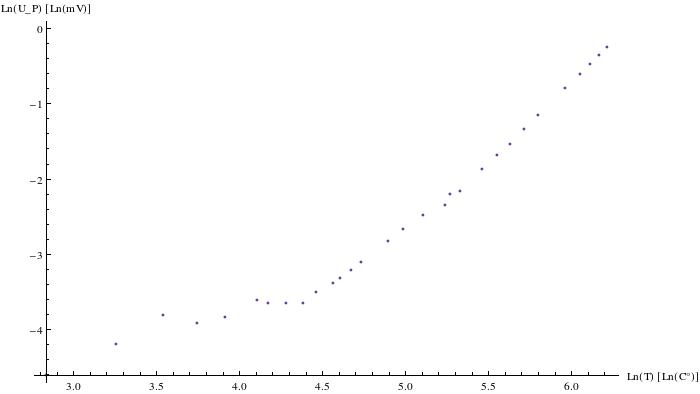
\includegraphics[scale=.6]{bilder/s_b_1.jpeg} 
		\caption{Grafik Messwerte}
	\end{figure}
	
Man sieht sofort, dass die Werte zu Beginn der Messung nicht zu unserer Erwartung und zu den restlichen Messwerten passen. Dies ist uns schon während der Messung aufgefallen, wobei uns die Betreuerin mitteilte, dass dies nicht unüblich sei. Trotzdem haben wir darauf hin die Ausrichtung der Lochblende verändert, damit die Strahlung besser auf die Thermosäule treffen konnte. Dies liegt daran, dass die Körper der Betreuer und Stunden ebenfalls strahlen, was im niedrigen Temperaturbereich höhere Störungen hervorrufen. Außerdem könnten die Messungen vom "`Wärmeleitung"'-Versuch beeinflusst worden sein. Danach schien der Verlauf der Messung eher unserer Erwartung zu entsprechen. Um einen sinnvollen Wert zu erhalten, lassen wir deshalb die "`unpassenden"' Werte zu Beginn der Messung wegfallen bei der linearen Regression. So erhalten wir:

\begin{figure}[H]
		\centering
		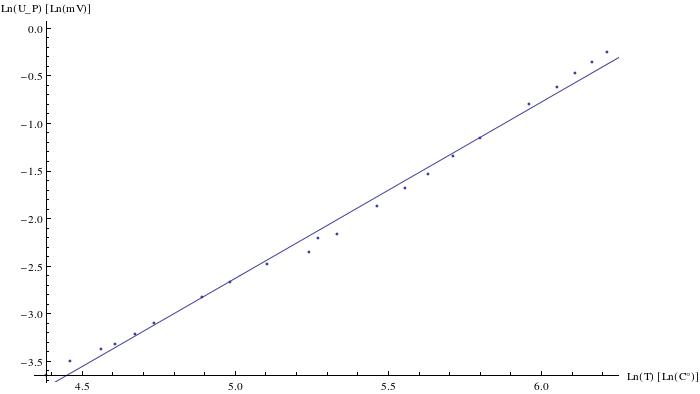
\includegraphics[scale=.6]{bilder/s_b_2.jpeg} 
		\caption{Lineare Regression}
	\end{figure}

Als Steigung liefert uns Mathematica m= 1.86. Dieser Wert weicht leider sehr stark ($\unit[53.5]{\%}$) vom erwarteten Wert 4 ab. Die starke Abweichung könnte damit zusammenhängen, dass wir an der Thermosäule, trotz der geänderten Ausrichtung nur sehr geringe Werte aufnahmen, was darauf schließen lässt, dass der Strahler eventuell nicht mehr richtig strahlt. Eventuell könnte die Messung auch durch die Änderung der Ausrichtung der Lochblende beeinflusst worden sein.

\section{Emissionsvermögen}

In diesem Versuch sollte das Emissionsvermögen verschiedener Materialien untersucht werden. Dazu wurde ein ähnlicher Aufbau wie in der vorherigen Aufgabe verwendet. Allerdings diente als Strahlungsquelle anstatt eines schwarzen Strahlers, eine Kreisscheibe die in verschiedene Sektoren mit jeweils unterschiedlichen Materialien (bzw. Beschichtungen). Zur Messung der Temperatur der Scheibe wurde wiederum ein Thermoelement verwendet, allerdings diente dieses Mal ein Eisbecken (also $\unit[0]{C^\circ}$) als Referenztemperatur, weshalb wir aus der Messung auch die tatsächliche Temperatur der Scheibe erhielten. Dazu wurde wiederum mit eine Tabelle der Spannungswert in einen Temperaturwert umgerechnet.\\ \\
Bei der Messung wurde folgendermaßen vorgegangen: Die Kreisscheibe wurde so nahe wie möglich vor der Lochblende platziert. Die Kreisscheibe war drehbar, so dass man nacheinander die verschiedenen Sektoren hinter der Lochblende einstellen konnte. Wir maßen für verschiedene Temperaturen die $U_P$-Werte der einzelnen Sektoren schnell nacheinander und notierten dann den Bereich der Temperaturänderung. Dabei erhielten wir folgende Werte:

\begin{table}[H]
\caption{Messwerte}
\tabcolsep=0.03cm
	\begin{tabular}{c|c|c|c|c|c}
   $U_{Th}$ (mV) & $T $ (C$^\circ) $  & $U_P$ Cu(blank) (mV) & $U_P$ Cu(aufgeraut) (mV) & $U_P$ Ruß (mV) & $U_P$ TiO (mV)\\
		\hline
		 1.35-1.5 & 33.5 & 0.008 & 0.0025 & 0.009 & -0.003\\
		 1.7-1.8 & 42 & 0.009 & 0.002 & 0.007 & -0.012\\
		 2.2-2.35 & 54-55 & 0.009 & 0.004 & 0.055 & -0.027\\
		 2.45-2.75 & 60-67 & 0.011 & -0.018 & 0.007 & -0.039\\
		 2.95-3.1 & 71-76 & 0.009 & -0.02 & 0 & -0.054\\
		 3.15-3.25 & 77-79.8 & 0.001 & -0.029 & -0.004 & -0.069\\
		 3.3-3.4 & 81-83.3 & 0.0009 & -0.0295 & -0.0075 & -0.0755\\
		 3.5-3.55 & 85.5-87 & 0 & -0.031 & -0.008 & -0.083\\
		 3.6-3.65 & 88-89 & 0.0015 & -0.0305 & -0.009 & -0.0835\\
		 3.85-3.9 & 94-95 & 0 & -0.046 & -0.01 & -0.0975\\
		 4-4.2 & 98-102.5 & -0.003 & -0.048 & -0.01356 & -0.109\\
	\end{tabular}
\end{table}
Man sieht schnell, dass die Messwerte unseren Erwartungen nicht entsprechen. Zu Beginn der Messung hatten die Spannung der meisten Materialien ein anderes Vorzeichen, als im weiteren Verlauf. Wir gehen davon aus, dass nur die Werte mit negativem Vorzeichen verwendet werden sollten. Bei den positiven Werten könnte es sein, dass es zu einer Beeinflussung durch die Umgebung kam, da diese Werte in einem niedrigeren Temperaturbereich auftraten. Störquellen könnten z.B. aus dem Parallelversuch gekommen sein. Des weiteren scheint das blanke Kupfer beschädigt zu sein, da die Werte dafür überhaupt nicht einzuordnen sind. Wir verwenden zur Auswertung also nur die sinnvoll erscheinenden Werte.\\
Damit können wir nun nochmals die $U_P-T^4$-Abhängigkeit des Stefan-Boltzmann-Gesetzes nachweisen. Wobei für einen nicht schwarzen Strahler gilt $P= \epsilon \cdot \sigma \cdot A \cdot T^4$.
\begin{figure}[H]
		\centering
		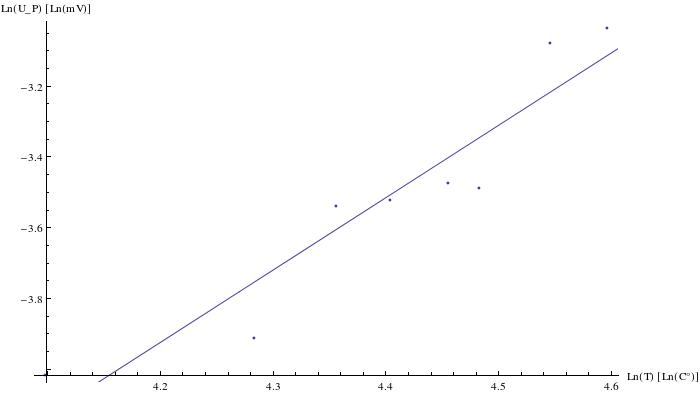
\includegraphics[scale=.6]{bilder/waerme_2_cu.jpeg} 
		\caption{aufgerautes Kupfer}
	\end{figure}
	\begin{figure}[H]
		\centering
		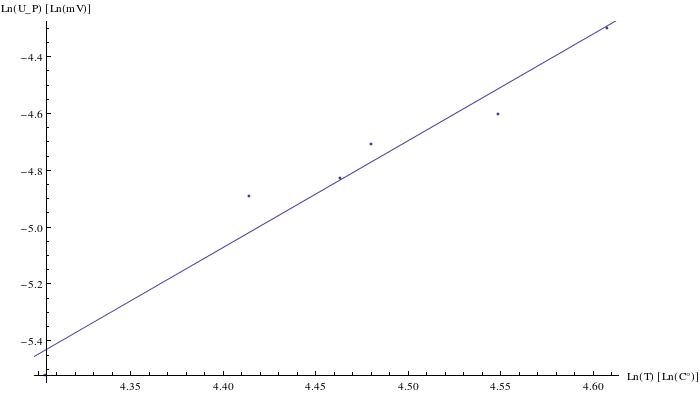
\includegraphics[scale=.6]{bilder/waerme_1_ru.jpeg} 
		\caption{Ruß}
	\end{figure}
\begin{figure}[H]
		\centering
		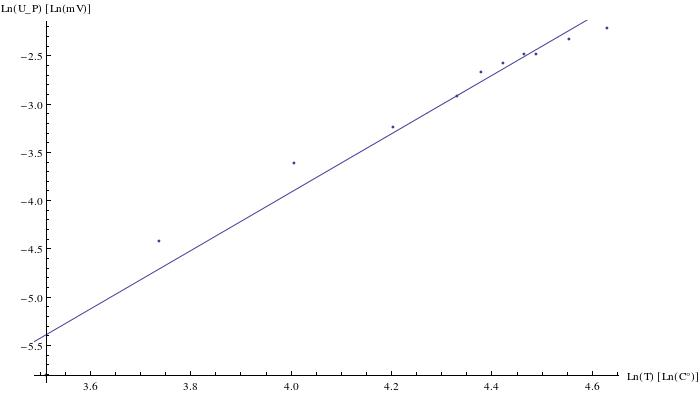
\includegraphics[scale=.6]{bilder/waerme_2_ti.jpeg} 
		\caption{Titanoxid}
	\end{figure}
	Man kann in den Schaubildern eine gewisse Linearität erkennen, allerdings haben wir nur wenige brauchbare Messwerte verwenden können, weshalb die Aussagekraft der Schaubilder nicht sonderlich groß ist. Als Steigungen erhalten wir $m_{cu}$= 2.05, $m_{Ruß}$= 3.7 und  $m_{Ti}$= 3.02. Der Wert für Ruß ist dabei sogar recht nahe am Theoriewert ( $\unit[7.5]{\%}$ Abweichung), allerdings wie eben erwähnt nicht sehr aussagekräftig. Die Werte für raues Kupfer (Abweichung $\unit[44.7]{\%}$) und Titanoxid (Abweichung $\unit[24.5]{\%}$) weichen stark von der Theorie ab. Trotzdem konnte man bei diesen 3 Materialien eine Linearität erkennen. Wir haben versuchsweise die Werte für blankes Kupfer ebenfalls in ein Schaubild eingetragen, diese waren aber nicht annähernd linear und scheinen komplett unbrauchbar, deshalb lassen wir sie auch bei der Betrachtung des Emissionsvermögen weg.
\begin{figure}[H]
		\centering
		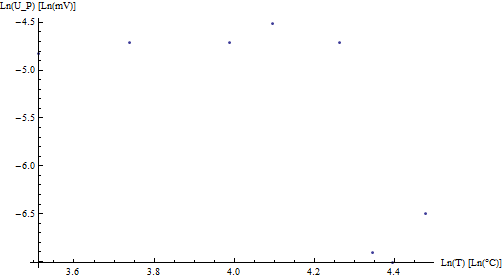
\includegraphics[width=0.6\textwidth]{bilder/warme_2_blank_cu.png} 
		\caption{Blankes Kupfer}
	\end{figure}
Nun wollen wir das Emissionsvermögen $E$ bestimmten. Wie aus der Vorbereitung bekannt, ist dieses definiert als Quotient der abgestrahlten Leistung des Sektors und der abgestrahlten Leistung eines schwarzen Strahlers bei gleiche Temperatur $E = \frac{P_{Sek}}{P_S}$. Da wir in diesem Versuch keinen schwarzen Strahler als Referenz haben, verwenden wir stattdessen die Werte von Titanoxid, da dies am nächsten an den schwarzen Strahler heran kommt. Nun trägt man die gemessenen Spannung der anderen Sektoren über die Spannung von Titanoxid auf und erhält aus der Steigung der Regressionsgeraden den Emissionskoeffizienten.
\begin{figure}[H]
		\centering
		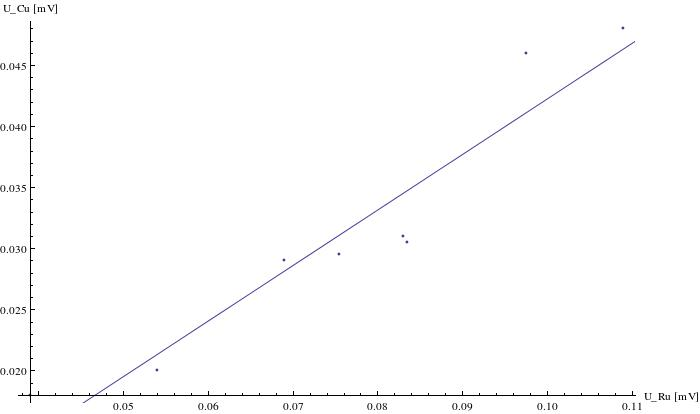
\includegraphics[scale=.6]{bilder/waerme_2_2_cu.jpeg} 
		\caption{Emissionsvermögen für raues Kupfer}
	\end{figure}
	
\begin{figure}[H]
		\centering
		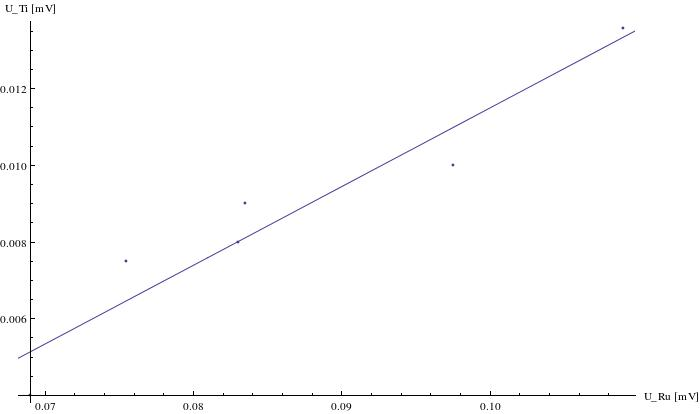
\includegraphics[scale=.6]{bilder/waerme_2_2_ru.jpeg} 
		\caption{Emissionsvermögen Ruß}
	\end{figure}
	
	Wir erhalten für die Steigung und somit für das Emissionsvermögen:
	
\begin{table}[H]
\centering
\caption{Emissionsvermögen der Materialien}
	\begin{tabular}{c|c|c}
   aufgerautes Kupfer & Ruß & Titanoxid\\
		\hline
	 0.454 & 0.205 & 1
	\end{tabular}
\end{table}

Titanoxid hat hier definitionsgemäß den Wert 1, d.h. da die anderen Werte kleiner sind, hat Titanoxid das höchste Emissionsvermögen. Man sieht schon in den Schaubildern, dass die Linearität nur bedingt gegeben ist. Auch dass der Wert für Ruß kleiner ist als der für raues Kupfer, ist physikalisch wenig sinnvoll, da raues Kupfer besser reflektiert als eine berußte Fläche und damit schlechter Wärme absorbiert. Absorption- und Emissionsvermögen sind proportional, also bedeutet schlechtere Absorption schlechtere Emission. Insgesamt stimmen die Messwerte mit den Erwartungen nicht überein. Woran dies genau liegt, können wir nicht sagen. Eventuell sind Teile des Versuchsaufbau schadhaft.

\section{Temperatur einer Glühlampe}

In diesem Versuch sollte die Temperatur einer Glühlampe bzw. des Glühwendels im Innern der Glühlampe mit einem optischen Pyrometer als Messgerät bestimmt werden. Die Funktionsweise eines solchen Pyrometers wurde in der Vorbereitung bereits besprochen, allerdings gab es im Versuch einen Unterschied zur theoretischen Arbeitsweise: Der Glühwendel der Lampe wurde nicht direkt in die Ebene des Glühwendels des Pyrometers projektiert, sonder war als roter Lichtpunkt neben dem Glühwendel des Pyrometers zu sehen. Somit konnte man durch das Regeln des Pyrometerstroms (und somit der Temperatur bzw. Strahlung) den Lichtpunkt nicht verschwinden lassen. Es war statt dessen erforderlich das Pyrometer so einzustellen, dass Lichtpunkt und Glühwendel die gleiche Helligkeit haben. Der dazu verwendete Pyrometerstrom ist dann, wie in der Vorbereitung beschrieben, charakteristisch für die Temperatur der Glühlampe (bzw. des Glühwendels). Hier sei angemerkt, dass der Glühwendel in der Lampe wohl ebenfalls aus Wolfram besteht, da sonst ein Vergleich der Helligkeit wenig sinnvoll wäre.\\
Da diese Methode sehr subjektiv ist (vor Allem, da der Lichtpunkt nicht wirklich verschwindet), wurde die Messung immer von der selben Person durchgeführt. Folgende Tabelle enthält unsere gemessenen Werte:

\begin{table}[H]
\centering
\caption{Messwerte}
	\begin{tabular}{c|c}
   $I_{Lampe}$ (A) & $I_{Pyro}$ (A)\\
		\hline
	 2.51 & 2.29\\
	 2.75 & 2.63\\
	 3.09 & 2.88\\
	 3.25 & 2.99\\
	 3.50 & 3.29\\
	 3.76 & 3.50\\
	 4.00 & 3.87\\
	\end{tabular}
\end{table}

Mit Hilfe einer gegebenen Tabelle, lassen sich die Stromwerte in Temperaturwerte umrechnen. Die Temperatur die sich dabei ergibt ist allerdings noch nicht die tatsächliche Temperatur der Lampe (bzw. Glühwendels) sondern die schwarz Temperatur $T_S$ (siehe Vorbereitung). Allerdings gibt uns die Tabelle auch die Differenz $\Delta T = T_W - T_S$, zwischen der wahren Temperatur $T_W$ und der schwarz Temperatur an, womit wir aus der Summe die wahre Temperatur erhalten. Es ergibt sich damit:

\begin{table}[H]
\centering
\caption{Messwerte}
	\begin{tabular}{c|c|c|c}
   $I_{Lampe}$ (A) & $T_S$ (K) & $\Delta T$ (K) & $T_W$ (K)\\
		\hline
	 2.51 & 1600 & 102 & 1702\\
	 2.75 & 1795 & 132 & 1927\\
	 3.09 & 1930 & 154 & 2084\\
	 3.25 & 1975 & 162 & 2137\\
	 3.50 & 2110 & 186 & 2296\\
	 3.76 & 2200 & 205 & 2405\\
	 4.00 & 2350 & 237 & 2587\\
	\end{tabular}
\end{table}

Da die Temperatur der Lampe linear von dem Lampenstrom abhängig sein sollte, überprüfen wir dies indem wir ein Diagramm erstellen.

\begin{figure}[H]
		\centering
		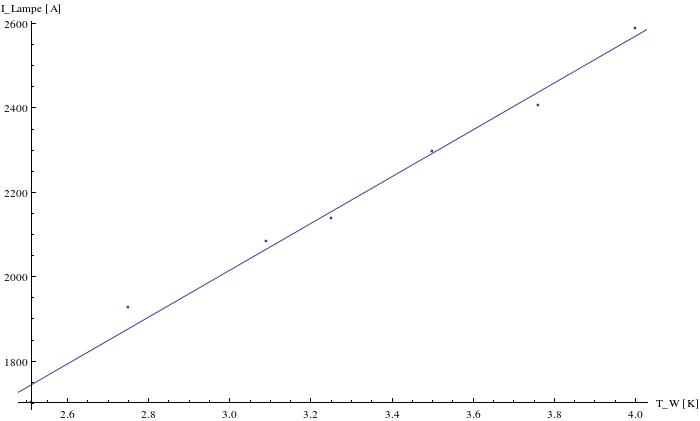
\includegraphics[scale=.6]{bilder/waerme_3.jpeg} 
		\caption{Linearität der wahren Temperatur}
	\end{figure}
  
  Auch wenn wir recht wenige Werte hier haben, sieht man doch relativ deutlich eine lineare Abhängigkeit.
\end{document}